\documentclass[paper=letter,fontsize=11pt]{scrartcl} % KOMA-article class

\usepackage[english]{babel}
\usepackage[utf8x]{inputenc}
\usepackage[protrusion=true,expansion=true]{microtype}
\usepackage{amsmath,amsfonts,amsthm}     % Math packages
\usepackage{graphicx}                    % Enable pdflatex
\usepackage[svgnames]{xcolor}            % Colors by their 'svgnames'
\usepackage{geometry}
%\textheight=700px                    % Saving trees ;-)
%\usepackage{url}
\usepackage[colorlinks=true,
linkcolor=blue,
urlcolor=blue]{hyperref}
\usepackage{float}
\usepackage{etaremune}
\usepackage{wrapfig}
\usepackage{multicol}

\usepackage{comment}

\usepackage{attachfile}

\frenchspacing              % Better looking spacings after periods
\pagestyle{empty}           % No pagenumbers/headers/footers

%\addtolength{\voffset}{-40pt}
%\addtolength{\textheight}{20pt}

\setlength\topmargin{0pt}
\addtolength\topmargin{-\headheight}
\addtolength\topmargin{-\headsep}
\setlength\oddsidemargin{0pt}
\setlength\textwidth{\paperwidth}
\addtolength\textwidth{-2in}
\setlength\textheight{\paperheight}
%\addtolength\textheight{-3in}
\addtolength\textheight{-2in}
\usepackage{layout}

%%% Custom sectioning}{sectsty package)
%%% ------------------------------------------------------------
\usepackage{sectsty}

\sectionfont{%			            % Change font of \section command
	\usefont{OT1}{phv}{b}{n}%		% bch-b-n: CharterBT-Bold font
	\sectionrule{0pt}{0pt}{-5pt}{1pt}}

%%% Macros
%%% ------------------------------------------------------------
\newlength{\spacebox}
\settowidth{\spacebox}{8888888888}			% Box to align text
\newcommand{\sepspace}{\vspace*{1em}}		% Vertical space macro

\newcommand{\MyName}[1]{ % Name
		\Huge \usefont{OT1}{phv}{b}{n} \hfill #1
		\par \normalsize \normalfont}
		
\newcommand{\MySlogan}[1]{ % Slogan}{optional)
		\large \usefont{OT1}{phv}{m}{n}\hfill \textit{#1}
		\par \normalsize \normalfont}

\newcommand{\NewPart}[2]{\section*{\uppercase{#1} \small \normalfont #2}}

\newcommand{\NewParttwo}[1]{
		\noindent \huge \textbf{#1}
        \normalsize \par}



\newcommand{\PersonalEntry}[2]{\small
		\noindent\hangindent=2em\hangafter=0 % Indentation
		\parbox{\spacebox}{        % Box to align text
		\textit{#1}}		       % Entry name}{birth, address, etc.)
		\small\hspace{1.5em} #2 \par}    % Entry value

\newcommand{\SkillsEntry}[2]{      % Same as \PersonalEntry
		\noindent\hangindent=2em\hangafter=0 % Indentation
		\parbox{\spacebox}{        % Box to align text
		\textsf{#1}}			   % Entry name}{birth, address, etc.)
		\hspace{1.5em} #2 \par}    % Entry value	
		
\newcommand{\EducationEntry}[4]{
		\noindent \textbf{#1} \hfill      % Study
		\colorbox{White}{%
			\parbox{6em}{%
			\hfill\color{Black}#2}} \par  % Duration
		\noindent \textit{#3} \par        % School
		\noindent\hangindent=2em\hangafter=0 \small #4 % Description
		\normalsize \par}

\newcommand{\WorkEntry}[5]{
		\noindent \textbf{#1}
        \noindent \small \textit{#2}
        \hfill      % Study
        \colorbox{White}{%
			\parbox{6em}{%
			\hfill\color{Black}#3}} \par  % Duration
		\noindent \textit{#4} \par        % School
		\noindent\hangindent=2em\hangafter=0 \small #5 % Description
		\normalsize \par}

\newcommand{\Language}[2]{
		\noindent \textbf{#1}
        \noindent \small \textit{#2}}
        
\newcommand{\Text}[1]{\par       
		\noindent \small #1 
		\normalsize \par}
        
\newcommand{\Textlong}[4]{
		\noindent \textbf{#1} \par
        \sepspace
        \noindent \small #2
        \par\sepspace      
		\noindent \small #3
        \par\sepspace      
		\noindent \small #4
        \normalsize \par}
        
\newcommand{\JobSkills}[2]{
		\noindent #1,
		
}
	    
              

\newcommand{\PaperEntry}[7]{
		\noindent #1, ``\href{#7}{#2}", \textit{#3} \textbf{#4}, #5 (#6).}


\newcommand{\ArxivEntry}[3]{
		\noindent #1, ``\href{http://arxiv.org/abs/#3}{#2}", \textit{{cond-mat/}#3}.}
        
\newcommand{\BookEntry}[4]{
		\noindent #1, ``\href{#3}{#4}", \textit{#3}.}
        
\newcommand{\FundingEntry}[5]{
        \noindent #1, ``#2", \$#3 (#4, #5).}

\newcommand{\TalkEntry}[4]{
		\noindent #1, #2, #3 #4}

\newcommand{\ThesisEntry}[5]{
		\noindent #1 -- #2 #3 ``#4" \textit{#5}}

\newcommand{\CourseEntry}[3]{
		\noindent \item{#1: \textbf{#2} \\ #3}}

%%% Begin Document
%%% ------------------------------------------------------------
\begin{document}

%\layout

% you can upload a photo and include it here...
\begin{wrapfigure}{l}{0.5\textwidth}
	\vspace*{-2em}
		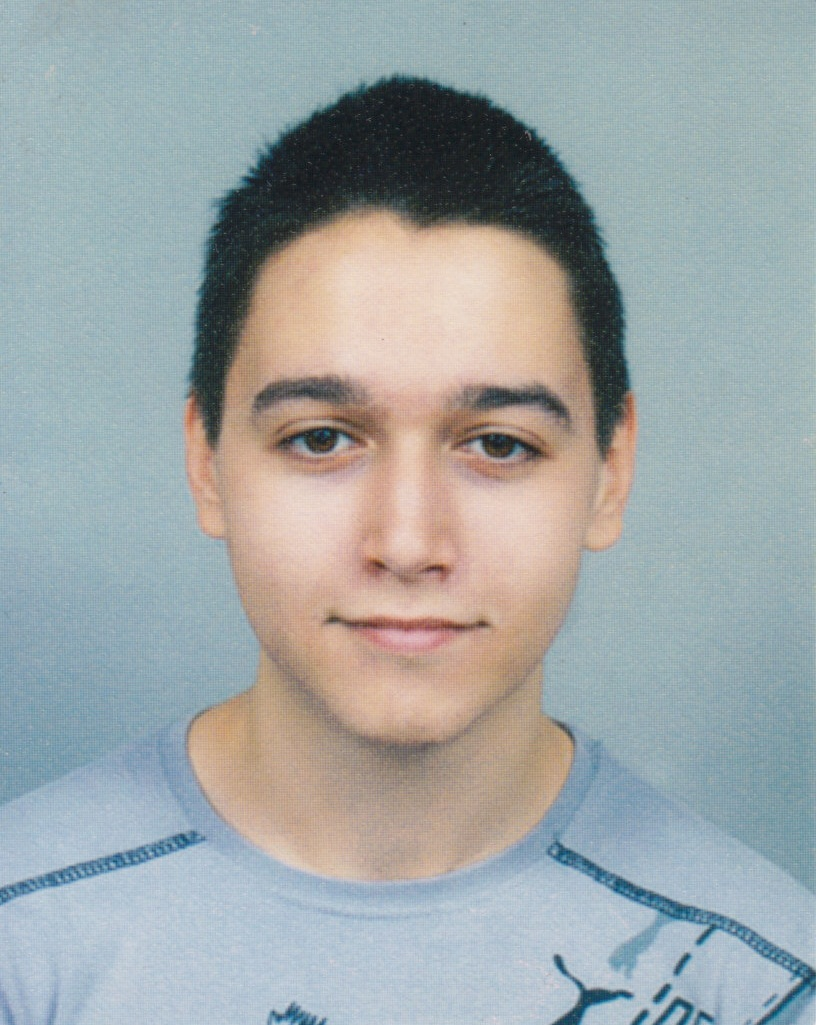
\includegraphics[width=0.15\textwidth]{IMG.jpg}
\end{wrapfigure}

\MyName{Boian Ivanov}
\MySlogan{Curriculum Vit\ae\ } %(\today)}

\sepspace
\sepspace

%%% Personal details
%%% ------------------------------------------------------------
\NewPart{}{}

\begin{multicols}{2}
\PersonalEntry{Address:}{{Lyulin 301}, 1336 Sofia}
\PersonalEntry{Phone:}{+ 359 (0)878448744}
\PersonalEntry{Born:}{27.05.1995}
\PersonalEntry{Nationality:}{Bulgarian, Greek}
\PersonalEntry{Mail:}{\href{mailto:boian.ivanov44@gmail.com}{boian.ivanov44@gmail.com}}
\PersonalEntry{GitHub:}{\href{https://github.com/boian-ivanov/}{github.com/boian-ivanov/}}
\PersonalEntry{LinkedIn:}{\href{https://bg.linkedin.com/in/boianivanov}{linkedin.com/in/BoianIvanov/}}
\PersonalEntry{}{}
\end{multicols}


%%% About Me
%%% ------------------------------------------------------------
\NewPart{About Me}{}
I am a Web Developer with experience in client-side and server-side technologies, mainly PHP and JavaScript. Currently working on the OpenCart platform, but that doesn't stop me from being interested in other programming methods. Always researching and developing something on the side, while working. Still my passion for my work is what drives me forward in life.

%%% Work experience
%%% ------------------------------------------------------------
\NewPart{Work Experience}{(Reference on demand)}

\WorkEntry{Sapir Bulgaria LTD}{\href{https://sapirshop.com/}{sapirshop.com}}{Present}{Sofia, Bulgaria}{Development and administration of e-commerce marketplace based on OpenCart. Module development on the platform.}

\sepspace

\WorkEntry{IT STEP Computer Academy}{\href{https://itstep.bg/}{itstep.bg}}{2016 - 2017}{Sofia, Bulgaria}{Computer Science Educator - Composing and teaching courses in software education.}

\sepspace

\WorkEntry{RS Consult}{\href{http://rsc.bg/}{rsc.bg}}{2016 - 2017}{Sofia, Bulgaria}{Web developer working with PHP, Laravel and OpenCart.}

\sepspace

\WorkEntry{ITR Services}{\href{http://itrservices.eu/}{itrservices.eu}}{2016}{Sofia, Bulgaria}{Web Development Intern. E-commerce development with Magento.}

\sepspace

%%% Education
%%% ------------------------------------------------------------
\NewPart{Education}{}


\EducationEntry{Computer Science and Informatics}
{2013-2017}
{New Bulgarian University, Sofia}
{\begin{itemize}
\item{On-going education in the field of Informatics with focus on Object oriented programming, Web-Programming and Advanced Mathematics}
\end{itemize}}

\sepspace
\newpage
\EducationEntry{Maintenance of computer systems, applications and networks
}{2011-2013}{Serres, Greece}{
\begin{itemize}\item{Basic knowledge in networking and programming}\end{itemize}}



%%% LANGUAGES
%%% ------------------------------------------------------------
\NewPart{LANGUAGES}{}

\Language{Bulgarian}{(mother tongue),}
\Language{Greek}{ (fluent),}
\Language{English}{(fluent),}
\Language{German}{(B1)}

%%% Other Skills
%%% ------------------------------------------------------------
\NewPart{OTHER QUALIFICATIONS}{}

\WorkEntry{Drivers license}{}{2015}{Sofia, Bulgaria}{Car (B,B1) and Motorbike(AM)}

\end{document}
